\subsubsection{Attività}
\label{sec:3.2.1}
	\paragraph{Verifica di un \gl{ticket}}
	\label{sec:3.2.1.1}
		Ogni qual volta un \gl{ticket} sarà contrassegnato come \textbf{Completato} il \RES {} procederà nel seguente modo: 
		\begin{itemize}
			\item crea un \gl{ticket} di verifica;
			\item lo assegna ad un \textbf{verificatore};
			\item non appena il \gl{ticket} viene contrassegnato come \textbf{Completato} imposta il tag del \gl{ticket} oggetto di verifica a \textbf{Verificato}.
		\end{itemize}
		\begin{figure}
			\centering
			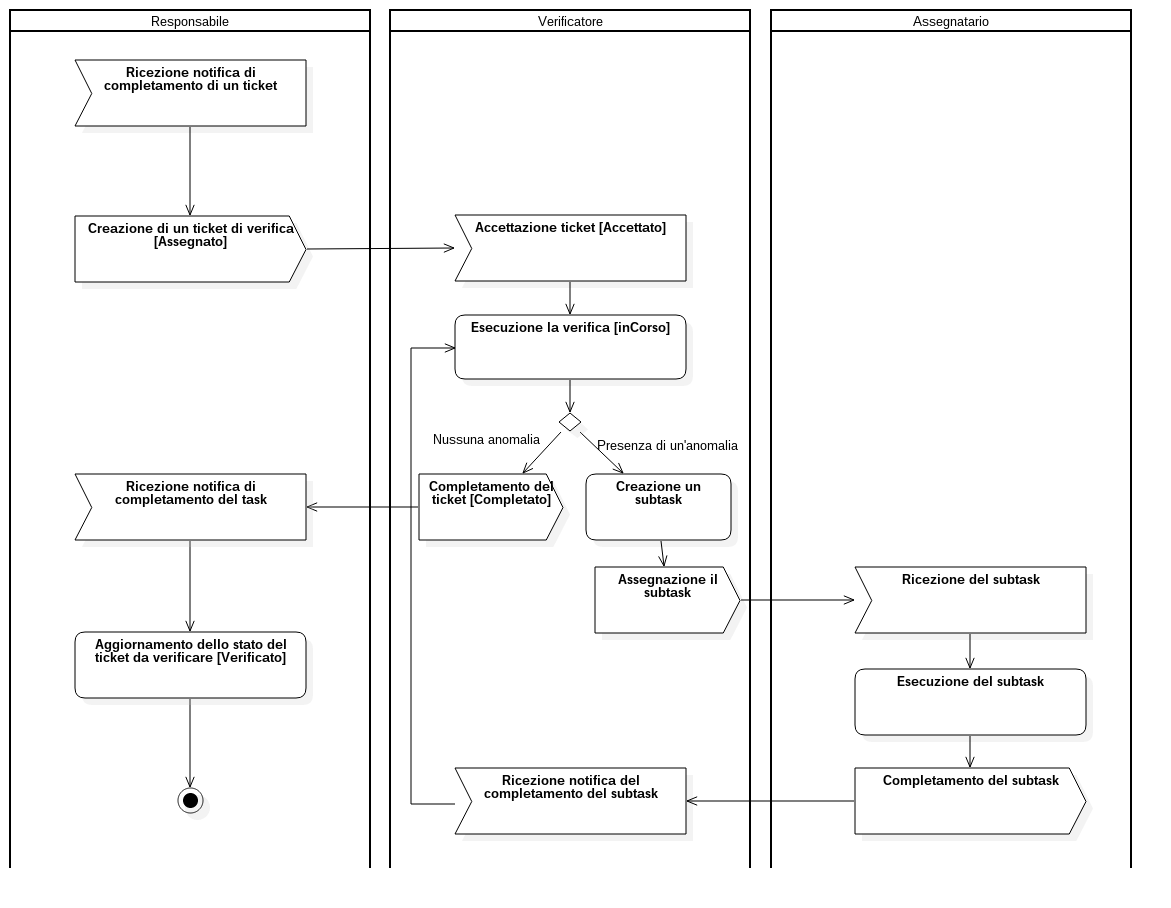
\includegraphics[scale=0.40]{img/ticketVerifica.png}
			\caption{Ticket di verifica}
		\end{figure}
	\paragraph{Analisi statica}
	\label{sec:3.2.1.2}
		L'analisi statica è una tecnica di verifica applicabile sia ai documenti che al codice. Verrà effettuata per tutta la fase di sviluppo del \gl{progetto} e serve per trovare anomalie, che verranno trattate come descritto nelle \NPdoc. Può essere applicata nei due modi seguenti.
			\subparagraph{Walkthrough}
			\label{sec:3.2.1.2.1}
				Consiste in una lettura del documento/codice cercando anomalie ed errori ad ampio spettro, cioè senza avere un'idea precisa di quali possibili errori si potranno trovare. Per evitare incomprensioni ogni modifica verrà discussa con gli autori e concordata tra le due parti. \\
				Il \gl{walkthrough}\ è una tecnica indispensabile nelle prime fasi di sviluppo, in cui non si ha un'idea precisa dei possibili errori. Usando questa tecnica sarà poi possibile stilare una ‘‘lista di controllo’’, dove verranno archiviati gli errori più frequenti. Tale lista sarà salvata nell'Appendice delle \NPdoc. \\ %quest'ultima frase sarà da decidere se tenere o no e quindi agire di conseguenza
				Inizialmente le fasi di verifica prevederanno perlopiù l'uso della tecnica \gl{walkthrough}. Appena la lista di controllo sarà sufficientemente ampia si userà sempre di più la tecnica di \gl{Inspection}.
			\subparagraph{Inspection}
			\label{sec:3.2.1.2.2}
				L'\gl{inspection}\ si basa sulla lettura mirata dei documenti/codice, cercando gli errori segnalati nella lista di controllo. Man mano che le verifiche procedono la lista verrà estesa e l'\gl{inspection}\ sarà più efficace.
	\paragraph{Analisi dinamica}
	\label{sec:3.2.1.3}
		L'analisi dinamica verifica il funzionamento delle sole componenti \gl{software} tramite dei test e aiuta ad identificarne le anomalie. \\
		Per garantire un risultato attendibile il test dev'essere ripetibile, ovvero deve ottenere sempre lo stesso output dallo stesso input quando viene eseguito nello stesso ambiente. Solo così il test garantisce di trovare eventuali problemi e quindi verificare la correttezza del \gl{prodotto} \gl{software}. \\
		Per ogni test deve essere definito:
		\begin{itemize}
			\item \textbf{ambiente:} è l'insieme dei sistemi \gl{hardware} e \gl{software} sui quali viene pianificata l'esecuzione del test sul \gl{prodotto}. Va inoltre specificato uno stato iniziale da cui il test deve partire;
			\item \textbf{specifica:} consiste nella specifica degli input e degli output attesi;
			\item \textbf{procedure:} è la specifica di ulteriori istruzioni sull'esecuzione del test e sull'interpretazione dei risultati.
		\end{itemize}
		Nelle prossime sezioni sono definiti i tipi di test effettuati sul \gl{prodotto} \gl{software} in sviluppo dal \gl{team}.
		\subparagraph{Test di unità}
		\label{sec:3.2.1.3.1}
			Il test di unità verifica che ogni singola unità di \gl{prodotto} funzioni correttamente. Per unità si intende una porzione di \gl{software} abbastanza piccola da poterne assegnare lo sviluppo ad un singolo \PR. \\
			Attraverso questo test verrà verificata la correttezza di ogni modulo base che compone il \gl{software}, limitando gli errori di implementazione. \\
			I test di unità sono identificati dalla seguente sintassi:
			\begin{center}
				TU[Codice test]
			\end{center}
		\subparagraph{Test di integrazione}
		\label{sec:3.2.1.3.2}
			Il test di integrazione verifica che due o più moduli già verificati funzionino come previsto quando vengono assemblati insieme. Inoltre aiuta a scovare i difetti residui sfuggiti dalla fase di test precedente. \\
			In più con questo test viene verificata la collaborazione tra i moduli prodotti e le componenti esterne usate come \gl{framework} o librerie. \\
			È possibile che vengano usate delle componenti ‘‘fittizie’’ al posto dei moduli non ancora completati per poter eseguire comunque dei test. \\
			I test di integrazione sono identificati dalla seguente sintassi:
			\begin{center}
				TI[identificativo del componente]
			\end{center}
			Tale identificativo corrisponde al componente i cui elementi sono integrati.
		\subparagraph{Test di sistema}
		\label{sec:3.2.1.3.3}
			I test di sistema validano l'intero \gl{prodotto} \gl{software} quando si ritiene che esso sia giunto ad una versione definitiva. Viene quindi controllato se tutti i requisiti sono stati soddisfatti. \\
			I test di sistema sono identificati dalla seguente sintassi:
			\begin{center}
				TS[Tipo Requisito][Codice Requisito]
			\end{center}
			Il tipo e il codice si riferiscono al requisito di cui verrà testato il soddisfacimento.
		\subparagraph{Test di regressione}
		\label{sec:3.2.1.3.4}
			Questo test viene eseguito dopo la modifica di una componente, e consiste nel rieseguire tutti i test. In questo modo si controlla che dopo la modifica tutti i moduli continuino a funzionare correttamente. \\
			Il tracciamento aiuta a capire quali sono i test da ripetere (di ogni tipo) poiché potenzialmente a rischio in caso di modifica.
		\subparagraph{Test di validazione}
		\label{sec:3.2.1.3.5}
			Coincide con il collaudo del \gl{software} in presenza del \gl{proponente}. Se il test risulta positivo il \gl{prodotto} sarà considerato sufficientemente maturo da permetterne il rilascio. \\
			I test di validazione sono identificati dalla seguente sintassi:
			\begin{center}
				TV[Tipo Requisito][Codice Requisito]
			\end{center}
			Il tipo e il codice si riferiscono al requisito di cui verrà testato il soddisfacimento.
	\paragraph{Tracciamento}
	\label{sec:3.2.1.4}
		Sarà compito dei Verificatori controllare la corrispondenza di ogni requisito con una o più fonti. In caso di anomalie bisogna comportarsi come descritto nella sezione 3.2.2.1. %aggiungere riferimento
\subsubsection{Procedure}
\label{sec:3.2.2}
	\paragraph{Gestione delle anomalie}
	\label{sec:3.2.2.1}
			Il \textbf{validatore} qualora riscontrasse delle anomalie procederà secondo la seguente procedura:
			\begin{itemize}
				\item crea un nuovo \gl{subtask} del \gl{ticket} di verifica per ogni anomalia riscontrata;
				\item assegna un titolo breve e preciso ad ogni \gl{subtask};
				\item se necessario aggiunge un commento che descriva l'anomalia riscontrata;
				\item assegna i subtasks al redattore del documento.
			\end{itemize}